\chapter{Proposta de solução}

Neste capítulo serão apresentados os componentes e procedimentos utilizados na elaboração da proposta de solução, denominada ``BURI''. Conforme as
etapas definidas na metodologia, ocorre inicialmente a discussão sobre a fase de pesquisa na Seção \ref{fase1}, seguida pela especificação 
das funcionalidades e comportamento do sistema BURI, contextualizados na Seção \ref{fase2}. O particionamento e execução de atividades nas áreas de 
\textit{hardware} e \textit{software} são explicados nas Seções \ref{fase3} e \ref{fase4}, respectivamente. Na Seção \ref{fase5},  o aplicativo Android e o 
dispositivo físico são avaliados por um grupo selecionado de alunos, a fim de garantir a usabilidade do sistema proposto e, posteriormente, são produzidas a documentação 
do projeto e guia de instalação na Seção \ref{fase6}. 

\section{Pesquisa}\label{fase1}

A primeira fase consiste na compreensão do problema. O objetivo é encontrar trabalhos semelhantes sobre o uso de IoT no monitoramento da qualidade do ar, assim 
como as consequências fisiológicas de inalação prolongada de monóxido de carbono, e identificar, através de um questionário aplicado aos alunos, as preocupações relacionadas 
ao tema no ambiente doméstico.

Em primeiro lugar, realizou-se uma revisão da literatura para identificar pesquisas no âmbito de tecnologias IoT e monitoramento do ar com foco 
em prevenção de acidentes, porém foram selecionados cinco trabalhos acadêmicos para o desenvolvimento da proposta e comparação de funcionalidades. 
Além disso, o estudo da intoxicação por monóxido de carbono visa investigar as consequências para a saúde humana. Portanto, a explicação científica sobre o tema é do 
artigo ``Carbon monoxide poisoning: a review for clinicians'' \cite{carbon-monoxide-poisoning-varon}, pois o conteúdo inclui 
explicação técnica e didática do processo de envenenamento, consequências no sistema neurológico e cardiovascular, fontes de contaminação e métodos de tratamento utilizados na medicina.

Por fim, foi aplicado um questionário a um grupo de estudantes da Escola Superior de Tecnologia da Universidade do Estado do Amazonas (EST/UEA), para coletar informações acerca de suas
preocupações em relação à qualidade do ar no ambiente doméstico. A pesquisa teve como propósito identificar as características do ambiente residencial desses alunos e avaliar seu 
nível de conscientização sobre os riscos associados aos poluentes atmosféricos. Participaram deste levantamento inicial 58 estudantes matriculados em cursos da área de Engenharia, os quais responderam 
ao questionário de forma voluntária.

As respostas do questionário são relevantes para a construção do protótipo. Como destaque, algumas informações importantes serão analisadas a seguir. Segundo a pesquisa, 
75,9\% dos estudantes utilizam um \textit{smartphone} com 
Sistema Operacional Android, pois a tecnologia é fonte de acesso à informação e inclusão digital no Brasil \cite{impacto-android-brasil}. Outro aspecto analisado foi 
a percepção dos alunos em relação à qualidade do ar em suas residências e arredores. Nas respostas, os relatos sobre a presença de fumaça e dificuldade respiratória em dias específicos foram comuns. Como relatou um dos alunos: ``a fumaça se tornou um problema pra resolver isso decidimos comprar um umidificador de ar''. 

Evidência do problema apresentado, a Universidade do Estado do Amazonas (UEA) suspende atividades presenciais nos dias 19 e 20 de setembro na capital e interior por causa 
da alta quantidade de poluentes, pois os índices ultrapassaram a marca de 125 $\mu m/m^{3}$ e um ar de boa qualidade permite a concentração de partículas em  até 25 $\mu m/m^{3}$ \cite{uea-queima-fecha}. Portanto, 
o funcionamento de um dispositivo de medição em tempo real com interface para dispositivo móvel representa uma boa alternativa para auxílio do usuário.

\begin{figure}[ht]
    \centering
    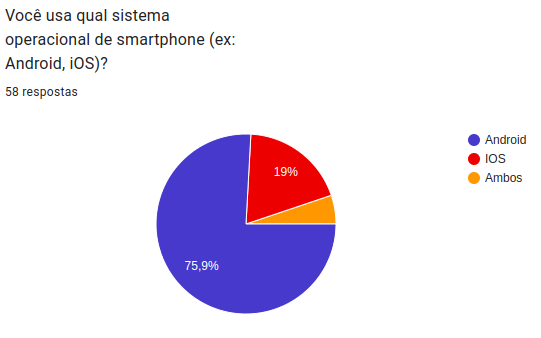
\includegraphics[width=.67\textwidth]{img/graf1-SO-smartphone.png}
    \caption{Sistemas Operacionais dos \textit{smartphones} dos alunos da EST. Fonte:Autor}\label{figSOsmartphone}
\end{figure}

Sobre o tipo de conexão com a internet, a figura \ref{figWifiAlunos} ilustra a porcentagem de estudantes com rede Wi-Fi em suas residências. De acordo com a pesquia,  
a maioria dos entrevistados possui acesso à rede Wi-Fi. Esse valor é especialmente útil para a viabilidade do projeto, uma vez que a conectividade permitirá o funcionamento do sistema no modo \textit{online}.

\begin{figure}[ht]
    \centering
    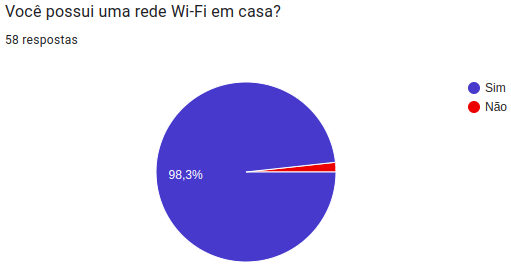
\includegraphics[width=.67\textwidth]{img/graf1-wifi.png}
    \caption{Uso de Wi-Fi dos alunos da EST. Fonte:Autor}\label{figWifiAlunos}
\end{figure}

O último levantamento refere-se às expectativas em relação ao \textit{hardware}, destacando a preocupação com o uso do equipamento. Observou-se que apenas 37,9\% dos 
alunos já utilizaram algum dispositivo de automação residencial. Dessa forma, a solução proposta deve priorizar configurações simples, voltadas para usuários 
sem experiência prévia. 


\section{Especificação}\label{fase2}

A especificação é a etapa onde são definidas as funcionalidades do sistema embarcado e a modelagem da arquitetura e comunicação entre 
seus componentes. A partir das respostas, foram identificadas as principais funcionalidades 
para o sistema BURI, pois o desenvolvimento do sistema deve garantir que o protótipo final atenda às demandas reais do
público alvo. A funcionalidade de monitoramento em tempo real recebeu o maior número de votos (89,7\%) entre os participantes, porém opções como alerta de risco, fácil instalação e 
manutenção mínima foram requisitos proporcionalmente solicitados no questionário. 

\begin{figure}[ht]
    \centering
    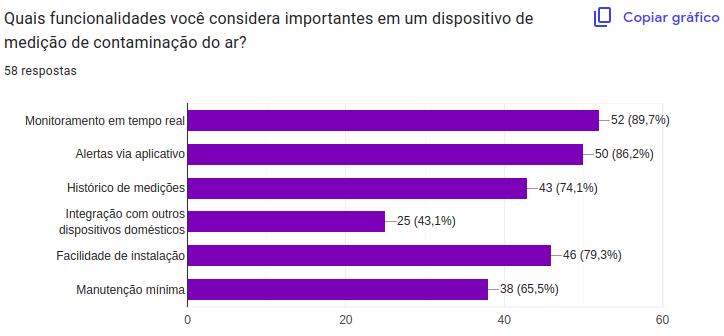
\includegraphics[width=.77\textwidth]{img/graf1-funcionalidades.png}
    \caption{Funcionalidades desejadas do sistema embarcado. Fonte:Autor}\label{figFuncionalidades}
\end{figure}

Com base nas sugestões dos estudantes e considerando o prazo de entrega do trabalho de conclusão de curso, o escopo da proposta de solução contempla a 
implementação das seguintes funcionalidades: modo \textit{online} e \textit{offline}, monitoramento em tempo real, alerta de risco por notificação e processo de instalação facilitado.
As funcionalidades apresentadas tem o objetivo de equilibrar a expectativa dos usuários e a viabilidade técnica, pois a estrutura considera os recursos disponíveis e o prazo definido no 
cronograma.

\section{Particionamento (Hw/Sw)}\label{fase3}

\section{Execução de Atividades}\label{fase4}

\section{Testes de aceitação}\label{fase5}

\section{Documentação}\label{fase6}